\documentclass[10pt]{article}
\usepackage{../../local}
\urlstyle{same}

\newcommand{\classcode}{EE 120}
\newcommand{\classname}{Signals and Systems}
\renewcommand{\maketitle}{%
\hrule height4pt
\large{Eric Du \hfill \classcode}
\newline
\large{HW 10} \Large{\hfill \classname \hfill} \large{\today}
\hrule height4pt \vskip .7em
\small{Header styling inspired by CS 70: \url{https://www.eecs70.org/}}
\normalsize
}
\linespread{1.1}
\begin{document}
	\maketitle
	\section*{Collaborators}	
	I worked with the following people on this assignment:
	\begin{itemize}
		\item Teja Nivarthi: 3036508567
		\item Nikhil Maserang: 3036978230
	\end{itemize}
	\pagebreak
	\section*{Problem 1}
	\begin{enumerate}[label=\alph*)]
		\item Determine the Laplace transform and the associated region of convergence for the following signals:
			\begin{enumerate}[label=\roman*)]
				\item \( x(t) = \delta(t - 1) \) 

					\begin{solution}
						Just do the integral:
						\[
						\int_{-\infty}^{\infty} \delta(t - 1)e^{-st} \diff t = e^{-s}
						\] 
						Since \( x(t) \) is a delta function, the ROC is over all \( s \).
					\end{solution}
				\item \( x(t) = e^{-t}\cos(2t)u(t) \) 

					\begin{solution}
						This is well known Laplace transform pair:
						\[
							e^{-at}\cos(\omega_0t)u(t) \overset{\mathcal L}{\longleftrightarrow}
							X(s) = \frac{s + a}{(s + a)^2 + \omega_0^2}
						\] 
						Therefore, applying it to this situation we have:  
						\[
						X(s) = \frac{s + 1}{(s + 1)^2 + 4}
						\] 
						This has an ROC of \( \Re(s) > -1 \). 
					\end{solution}
				\item \( x(t) = \sin(t) u(-t) \) 

					\begin{solution}
						It helps here to write out the integral:
						\[
							X(s) = \int_{-\infty}^{\infty} \sin(t) u(-t) e^{-st} \diff t 
						\] 
						Now, let \( t' = -t \), so the integral becomes:
						\[
						X(s) = -\int_{-\infty}^{\infty} \sin(-t') u(t') e^{st'} \diff t'
						\] 
						This is the Laplace transform of \( \sin(\omega_0 t)u(t) \) with \( \omega_0 = -1 \), 
						so:
						\[
						X(s) = \frac{s}{s^2 + 1}
						\] 
						except here, our ROC is \( \Re(s) < 0 \). 
					\end{solution}
			\end{enumerate}
		\item For each Laplace transform and region of convergence pair below, determine the function 
			in time, \( x(t) \):
			\begin{enumerate}[label=\alph*)]
				\item \( X(s) = \frac{s + 2}{(s+2)^2 + 1}, \Re(s) > -2 \) 

					\begin{solution}
						This is the same form as part (ii) from the previous part, so 
						we know that:
						\[
						x(t) = e^{-2t}\cos(t) u(t)
						\] 
					\end{solution}
				\item \( X(s) = \frac{s e^{-s}}{s^2 + 1}, \Re(s) > 0 \) 

					\begin{solution}
						Here, we will write this out as a product of two Laplace transforms:
						\[
						X(s) = e^{-s} \cdot \frac{s}{s^2 + 1} = X_1(s)X_2(s)
						\] 
						We define \( X_1(s) = e^{-s} \) and \( X_2(s) = \frac{s}{s^2 + 1} \). Then, by the 
						convolution theorem, we know that this corresponds to the Laplace transform of 
						the signal \( x_1(t) * x_2(t) \), where \( x_1, x_2 \) are the corresponding inverse 
						Laplace transforms. Both of these are well known pairs, so we have:
						\[
						x_1(t) = \cos(t) u(t) \quad x_2(t) = \delta(t - 1) 
						\] 
						Therefore:
						\[
						x(t) = x_1(t) * x_2(t) = \cos(t)u(t) * \delta(t - 1) = \cos(t - 1) u(t- 1)
						\] 
					\end{solution}
				\item \( X(s) = \frac{s}{(s^2+ 1)^2}, \Re(s) > 0 \)

					\begin{solution}
						Taking inspiration from the Ed post about this problem, we take the indefinite integral of this:
						\[
						\int X(s) \diff s = -\frac{1}{2}\frac{1}{s^2 + 1}
						\] 
						Then, we know that \( \frac{1}{s^2 + 1}\overset{\mathcal L}{\longleftrightarrow} 
						\sin(t) u(t)\), and since 
						\[
							-t x(t) \overset{\mathcal L}{\longleftrightarrow} \dv{X(s)}{s}
						\] 
						then we can conclude:
						\[
						x(t) = -\frac{t}{2}\sin(t) u(t)
						\] 
					\end{solution}
			\end{enumerate}
		\end{enumerate}
	\pagebreak
	\section*{Problem 2}
	Suppose the following facts are given about the signal \( x(t) \) with Laplace transform \( X(s) \):
	\begin{enumerate}[label=\alph*)]
		\item \( x(t) \) is real and even
		\item \( X(s) \) has four poles and no zeros in the finite \( s \)-plane. 
		\item \( X(s) \) has a pole at \( s = \frac{e^{j \pi /4}}{2} \) 
		\item \( \int_{-\infty}^{\infty} x(t) \diff t = 4  \)
	\end{enumerate}
	\textbf{Determine \( X(s) \) and the corersponding ROC.}

	\begin{solution}
		From the second condition, we can write out \( X(s) = \frac{N(s)}{D(s)} \), and since \( X(s) \) has
		no zeroes, then we know that \( N(s) \) is a constant. Further, since \( D(s) \) has four 
		poles, let them be labelled \( p_1, p_2, p_3, p_4 \), then we can write:
		\[
		X(s) = \frac{c}{(s - p_1)(s - p_2)(s - p_3)(s - p_4)}
		\] 
		From the third condition, we get one of the poles for free, WLOG let's let that be 
		\( p_1 = \frac{1}{2}e^{j \pi / 4} \). Since \( x(t)  \) is real, then we know that \( X(s)  \) 
		is conjugate symmetric (i.e. \( X(s) = X^{*}(s^{*}) \), meaning that if \( p_1 =\frac{1}{2} e^{j \pi / 4} \)
		is a pole, then \( -p_1 \) is also a pole, so \( p_2 = -\frac{1}{2}e^{j \pi / 4} \).

		Further, since \( x(t) \) is even, then we know that \( X(s) \) is even, meaning that flipping the real 
		part (which amounts to swapping the sign on the exponent) should also give us zeroes. This gives us 
		our last two zeroes: 
		\[
		p_3 = \frac{1}{2}e^{- j \pi / 4} \quad p_4 = -\frac{1}{2}e^{- j \pi /4}
		\] 
		Now, we use the final condition to find the value of \( c \). Plugging in \( s = 0 \), we notice that 
		the denominator will be the product of the poles. However, since the poles pair up to be conjugates of each 
		other, this means that they will annihilate each other to unity:
		\[
		X(0) = 4 = \frac{c}{p_1 p_2 p_3 p_4} = \frac{c}{1} \implies c= 4
		\] 
		Therefore:
		\[
		X(s) = \frac{4}{(s - \frac{1}{2}e^{- j \pi / 4})(s + \frac{1}{2}e^{- j \pi / 4})(s - \frac{1}{2}e^{j \pi / 4})
		(s + \frac{1}{2}e^{j \pi / 4})}
		\] 
		The corresponding ROC will have to be the entire complex plane except for these poles? I'm not too sure about 
		this but this feels right. 
	\end{solution}
	\pagebreak
	\section*{Problem 3}
	\begin{enumerate}[label=\alph*)]
		\item Let \( Z_1(s), Z_2(s), X(s), Y(s) \) denote the Laplace transforms of \( z_1(t), z_2(t), x(t), y(t) \), 
			respectively. Assume the system starts at rest, that is \( y(t), z_1(t), z_2(t), x(t) = 0
			\ \forall  t < 0\). Furthermore, assume \( y(0), z_1(0) \) and \( z_2(0) = 0 \). 
			Calculate the ratio \( H(s) = \frac{Y(s)}{X(s)} \). 
			\begin{align*}
				\dv{z_1(t)}{t} &= z_2(t) \\
				\dv{z_2(t)}{t} &= -a_0z_1(t) - a_1z_2(t) + x(t) \\
				y(t) &=  b_0z_1(t) + b_1z_2(t) 
			\end{align*}

			\begin{solution}
				We know that the following is a property of the Laplace transform (given that the initial 
				conditions for \( t < 0 \) are all zero):
				\[
					\dv{x(t)}{t} \overset{\mathcal L}{\longleftrightarrow} s X(s)
				\] 
				Since \( z_1(t) \) and \( z_2(t) \) are related by a derivative, then we know that 
				\( s Z_1(s) = Z_2(s) \). Then, we now take the Laplace transform of the second equation:
				\[
				s Z_2(s) = s^2 Z_1(s) = -a_0Z_1(s) - a_1Z_2(s) + X(s)
				\] 
				Solving for \( X(s) \), we get:
				\[
				X(s) = s^2Z_1(s) + a_0Z_1(s) + a_1s Z_1(s) = (s^2 + a_1s + a_0) Z_1(s) 
				\] 
				Similarly for \( Y(s) \), we have:
				\[
				Y(s) = b_0Z_1(s) + b_1s Z_1(s) = (b_0 + b_1s)Z_1(s)
				\] 
				Therefore, we can write \( H(s) \) in terms of the ratio now:
				\[
					H(s) = \frac{(b_0 + b_1s)Z_1(s)}{(s^2 + a_1s + a_0)Z_1(s)} = \frac{b_0 + b_1s}{s^2 + a_1s + a_0}
				\] 
			\end{solution}
		\item Consider the system described by the differential equation:
			\[
				\dv[2]{y(t)}{t} + 3\dv{y(t)}{t} + 2y(t) = x(t)
			\] 
			Use the (bilateral) Laplace transform to determine the output \( y(t) \) when the input 
			is \( x(t) = e^{-3t}u(t) \) and the initial conditions (\( t < 0 \)) are:
			\[
				x(t) = 0, \quad y(t) = \frac{5}{2}, \quad \dv{y(t)}{t} = -\frac{9}{2} \quad \text{for \( t < 0 \)}
			\] 

			\begin{solution}
				So we're asked to solve the differential equation
				\[
					\dv[2]{y(t)}{t} + 3\dv{y(t)}{t} + 2y(t) = e^{-3t}u(t)
				\] 
				We'll take the Laplace transform, but we need to be careful of initial conditions:
				\begin{align*}
					\dv{y(t)}{t} &\overset{\mathcal L}{\longleftrightarrow} s Y(s) - y(0^{-})\\
					\dv[2]{y(t)}{t} & \overset{\mathcal L}{\longleftrightarrow} s^2 Y(s) - s y(0^{-}) - \dot y(0^{-})
				\end{align*}
				We're given the initial conditions in the problem, so the differential equation becomes:
				\[
				s^2 Y(s) - sy(0^{-}) - \dot y(0^{-}) + 3\left( s Y(s) - y(0^{-}) \right)  + 2Y(s) = \frac{1}{s + 3}
				\] 
				Substituting in the initial conditions and isolating for \( Y(s) \), we have:
				\[
				Y(s) = \frac{5s^2 + 21s + 20}{2(s + 3)(s^2 + 3s + 2)} = \frac{5s^2 + 21s + 20}{2(s + 3)(s+2)(s+1)}
				\] 
				Using partial fraction decomposition (I got lazy and used a computer for this), we get:
				\[
				Y(s) = \frac{1}{s+1} + \frac{1}{s + 2} + \frac{1}{2(s + 3)}
				\] 
				These are all well-known Laplace pairs, so the corresponding \( y(t) \) is:
				\[
				y(t) = e^{-t}u(t) + e^{-2t}u(t) + \frac{1}{2}e^{-3t}u(t)
				\] 

			\end{solution}
	\end{enumerate}
	\pagebreak
	\section*{Problem 4}
	Consider the series RLC-circuit shown in the figure below, where \( x \) and \( y \) are the input and output 
	respectively. 
	%diagram
	\begin{center}
		\begin{circuitikz}[american, cute inductors]
			%\draw (0,0) to[isource] (0,3) -- (2,3) to[R] (2,0) -- (0,0);
			\draw (0, 0) -- (4, 0) to [R, l= $R$] (4, 2) to [C, l = $C$] (4, 3)
			to [L, l = $L$] (0, 3) to[vsource, l=$x(t)$] (0, 0);
			\draw[-o] (4, 0) -- (5, 0) node[right] {$-$};
			\draw[-o] (4, 3) -- (5, 3) node[right] {$+$};
			\draw node at (5, 1.5) {$y(t)$};
		\end{circuitikz}
	\end{center}

	The transfer function \( \hat{H}(s) \), with the particular input and output signals specified in the figure 
	above, is given by
	\[
	\hat{H}(s) = \frac{RCs + 1}{LC s^2 + RCs + 1}
	\] 
	Let \( R = 5, L = 1 \), and \( C = 1 / 6 \), in appropriate units. 
	\begin{enumerate}[label=\alph*)]
		\item Determine the linear, constant-coefficient differential equation that governs the input-output 
			behavior of the circuit. 

			\begin{solution}
				We have the equation from lecture that given a transfer function of the form:
				\[
				H(s) = \frac{Y(s)}{X(s)} = \frac{\sum_{k=0}^{M} b_k s^{k}}{\sum_{k=0}^{N} a_k s^{k}}
				\] 
				then this gives an LCCDE of the form:
				\[
					LC \dv[2]{y(t)}{t} + RC \dv{y(t)}{t} + y(t) = RC \dv{x(t)}{t} + x(t)	
				\] 
			\end{solution}
		\item Suppose \( y(t) = 0 \forall t < 0 \) and \( \dot y(0^{-}) = 0 \) and \( y(0^{-}) = 0 \). Let the 
			input signal be the unit step: \( x(t) = u(t) \). Determine a reasonably simple expression for 
			\( y_{\text{SS}}(t) \), the steady-state response of the circuit. 

			\begin{solution}
				Since all initial conditions are zero, then the Laplace transform properties change to:
				\begin{align*}
					\dv{y(t)}{t} &\overset{\mathcal L}{\longleftrightarrow} s Y(s)\\
					\dv[2]{y(t)}{t} & \overset{\mathcal L}{\longleftrightarrow} s^2 Y(s) 
				\end{align*}
				For the right hand side, we have the relation that \( \dv{u(t)}{t} = \delta(t) \), which transforms 
				as the unity, so after the Laplace transform the equation becomes:
				\[
				Y(s)(LCs^2 + RCs + 1) = RC + \frac{1}{s}\implies Y(s) = \frac{RC + \frac{1}{s}}{LCs^2 + RCs + 1}
				\] 
				Plugging in the values for \( L, R, C \), we have
				\[
				Y(s) = \frac{1}{s} + \frac{2}{2 + s} - \frac{3}{3+s}
				\] 
				So this gives:
				\[
				y_{\text{SS}}(t) = u(t) + 2e^{-2t}u(t) - 3e^{-3t}u(t) = u(t)(1 + 2e^{-2t} - 3e^{-3t})
				\] 
			\end{solution}
		\item Now supose the initial conditions are \( \dot y(0^{-}) = -5 \) and \( y(0^{-}) = 2 \). Determine 
			a reasonably simple expresion for \( y_{\text{ZIR}}(t) \), the zero-input response of the circuit. 
			This just means the system output when \( x(t) \) is zero. 

			It may interest you to know the following properties of the Laplace transform. If \( y(t) \leftrightarrow 
			\hat{\mathcal Y}(s)\), then 
			\begin{align*}
				\dot y(t) &\leftrightarrow s \hat{\mathcal Y}(s) - y(0^{-})\\
				\ddot y(t) &\leftrightarrow s^2 \hat{\mathcal Y}(s) - sy(0^{-}) - \dot y(0^{-})
			\end{align*}

			\begin{solution}
				Here we now have to care about the initial conditions, so now the full equation 
				in the \( s \)-domain looks like:
				\[
				LC(s^2 Y(s) + s y(0^{-}) - \dot y(0^{-}) + RC(sY(s) - y(0^{-}) + Y(s) = RC + \frac{1}{s}
				\] 
				Plugging in appropriate values for \( L, R, C \) and the initial conditions, we eventually 
				get (after some lengthy algebra): 
				\[
				Y(s) = \frac{3RC + 2LCs + 5LC + \frac{1}{s}}{LCs^2 + RCs + 1} = \frac{1}{s} + \frac{13}{2 + s} - 
				\frac{12}{3 + s}
				\] 
				Recognizing each of the pairs, we get:
				\[
				y_{\text{ZIR}}(t) = u(t) + 13 e^{-2t}u(t) - 12e^{-3t}u(t) = u(t)(1 + 13 e^{-2t} - 12 e^{-3t})
				\] 
			\end{solution}
	\end{enumerate}
	\pagebreak
	\section*{Problem 5}
	A proportional-integral-derivative (PID) controller has the general form
	\[
		x(t) = K_p e(t) + K_i \int_{-\infty}^{t} e(\tau) \diff \tau + K_d \dv{e(t)}{t}
	\] 
	where \( e(t) \) is the error signal (see box diagram below).
	% diagram

	\begin{center}
		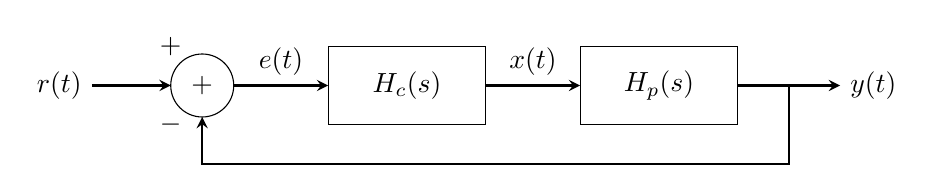
\begin{tikzpicture}
			\draw[-stealth, thick] (-3, 0) node[left] {\( r(t) \) } to (-2, 0);
			\draw (-1.6, 0) circle (0.4) node {\( + \) };
			\draw node at (-2, 0.5) {\( + \) };
			\draw node at (-2, -0.5) {\( - \) };
			\draw[-stealth, thick] (-1.2, 0) to node[midway, above] {\( e(t) \) } (0, 0); 
			\draw (0, -0.5) rectangle node {\( H_c(s) \) } ++(2, 1);
			\draw[-stealth, thick] (2, 0) to node[midway, above] {\( x(t) \) } (3.2, 0);
			\draw (3.2, -0.5) rectangle node {\( H_p(s) \) } ++(2, 1);
			\draw[-stealth, thick] (5.2, 0) to (6.5, 0) node[right]  {\( y(t) \) };
			\draw[-stealth, thick] (5.85, 0) -- (5.85, -1) -- (-1.6, -1) -- (-1.6, -0.4);
		\end{tikzpicture}
	\end{center}
	\begin{enumerate}[label=\alph*)]
		\item Find the transfer function \( H_c(s) = \frac{X(s)}{E(s)} \) of the PID controller. 

			\begin{solution}
				We take the Laplace transform of the given equation:
				\[
				X(s) = K_p E(s) + K_i \frac{1}{s}E(s) + K_d s E(s)
				\] 
				dividing through by \( E(s) \), we get:
				\[
				H_c(s) = K_p + \frac{K_i}{s} + K_d s
				\] 
			\end{solution}
		\item Find the closed-loop transfer function \( H(s) = \frac{Y(s)}{R(s)} \). 

			\begin{solution}
				From the diagram, we can tell that \( e(t) = r(t) - y(t) \), so this means that 
				\( E(s) = R(s) - Y(s) \). Then, we know that since these systems are connected in series, they are 
				linked together by a convolution:
				\[
				y(t) = e(t) * h_c(t) * h_p(t) \implies Y(s) = E(s) H_c(s) H_p(s) = R(s) H_c(s) H_p(s) - Y(s) H_c(s)
				H_p(s)
				\] 
				Dividing both sides by \( R(s) \), we get:
				\[
				\frac{Y(s)}{R(s)} = H_c(s) H_p(s) - \frac{Y(s)}{R(s)} H_c(s) H_p(s)
				\] 
				Therefore:
				\[
				H(s) = \frac{Y(s)}{R(s)} = \frac{H_c(s) H_p(s)}{1 + H_c(s) H_p(s)}
				\] 
			\end{solution}
		\item In many applications \( r(t) \) acts as a reference input, or the target value 
			we would like \( y(t) \) to reach. Suppose you have a purely proportional controller, 
			i.e., \( K_i = K_d = 0 \) and \( K_p > 0 \). What is the steady-state error 
			\( \lim_{t \to \infty}e(t) \) for a unit step input? 

			\begin{solution}
				Since \( K_i = K_d = 0 \), then this means that \( H_c(s) = K_p \), so we have:
				\[
				H(s) = \frac{K_p H_p(s)}{1 + K_p H_p(s)}
				\] 
				Further, for a unit step input, this implies that \( r(t) = u(t) \) and \( R(s) = \frac{1}{s} \). Thus,
				since \( E(s) = R(s) + H(s) R(s) \) (the second term comes from the feedback), we then know 
				that:
				\[
				E(s) = \frac{1}{s}\left( 1 + H(s) \right)  = \frac{1}{s}\left( 1 + \frac{K_p H_p(s)}{1 + K_p H_p(s)} \right) 
				\] 
				Now, the final value theorem states that the limit as \( t \to \infty \) for \( e(t) \) is 
				equivalent to finding \( \lim_{s \to 0}s E(s) \), so:
				\[
					\lim_{s \to 0} \frac{K_p H_p(s)}{1 + K_p H_p(s)} = \frac{K_p H_p(0)}{1 + K_p H_p(0)}
				\] 
				Without knowledge of \( H_p \), we cannot proceed further. 
			\end{solution}
		\item Now suppose you have a PI controller, i.e., \( K_d = 0 \) and 
			\( K_i, K_p > 0 \). What happens to the steady-state error?

			\begin{solution}
				If \( K_d = 0 \), then \( H_c(s) = K_p + \frac{K_i}{s} \). Following the same steps, we have:
				\[
					H(s) = \frac{K_p H_p(s) + \frac{K_i}{s} H_p(s)}{1 + K_p H_p(s) +\frac{K_i}{s}H_p(s)}
				\]
				Therefore:
				\[
				E(s) = \frac{1}{s}(1 + H(s)) = \frac{1}{s}\left(1 + \frac{K_p H_p(s) + \frac{K_i}{s} H_p(s)}{1 + K_p H_p(s) +\frac{K_i}{s}H_p(s)}\right)
				\] 
				Now, we can write this in a slightly easier to manipulate form, by factoring out \( \frac{1}{s} \) 
				from the numerator and denominator of the inner term:
				\[
				E(s) = \frac{1}{s}\left( 1 + \frac{(s K_p + K_i)H_p(s)}{s + (sK_p + K_i) H_p(s)} \right) 
				\] 
				Now, we can take \( \lim_{s \to 0}s E(s) \):
				\[
					\lim_{s \to 0} sE(s) = \lim_{s \to 0} 1 + \frac{(s K_p + K_i)H_p(s)}{s + (sK_p + K_i) H_p(s)} 
					=1 +  \frac{K_i H_p(0)}{K_i H_p(0)} = 2
				\] 
				so the steady-state error becomes constant. 
			\end{solution}
	\end{enumerate}
\end{document}
